% 2008 年湖南卷文科第 18 题：四棱锥 P-ABCD，底面菱形边长 1、∠BCD=60°，E 为 CD 中点，
%   PA ⊥ 底面，PA=√3。
% 来源 PDF：gaokaomath-src/普通高考/2008/2008湖南文.pdf
% SHA-256：481d0aaef90a5fb7309defcc13eb51333a625183edae799cd50a86bbac0c0dbe
% 原页：2008湖南文.pdf 第 1 页（A3 三栏）第 3 栏，书页码 455。
% 重绘依据：按原页斜投影：A 在左下、B 在其右侧、C 在最右、D 在 B 的后上方（被遮挡）；
%   P 在 A 的正上方。可见棱 PA、PB、PC、AB、BC 实线，被遮挡的 AD、DC 与 PD 虚线，
%   E 标在 DC 上。
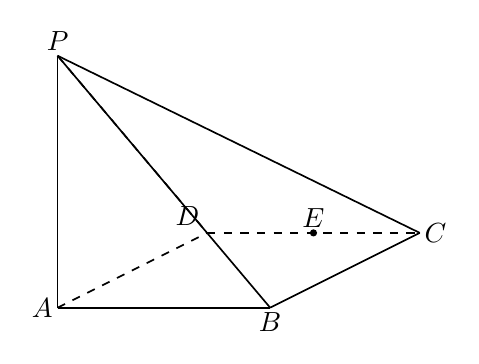
\begin{tikzpicture}[scale=1.0, semithick, every node/.style={inner sep=1.5pt}]
  \coordinate (A) at (0.00,0.00);
  \coordinate (B) at (2.70,0.00);
  \coordinate (C) at (4.60,0.95);
  \coordinate (D) at (1.90,0.95);
  \coordinate (P) at (0.00,3.20);

  % 可见棱
  \draw (P) -- (A);
  \draw (P) -- (B);
  \draw (P) -- (C);
  \draw (A) -- (B);
  \draw (B) -- (C);

  % 被遮挡的棱
  \draw[dashed] (P) -- (D);
  \draw[dashed] (A) -- (D);
  \draw[dashed] (D) -- (C);

  % CD 的中点 E
  \coordinate (E) at (3.25,0.95);
  \fill (E) circle (1.3pt);

  \node[left] at (A) {$A$};
  \node[below] at (B) {$B$};
  \node[right] at (C) {$C$};
  \node[above left=1pt] at (D) {$D$};
  \node[above] at (E) {$E$};
  \node[above] at (P) {$P$};
\end{tikzpicture}
